\documentclass{beamer}

\usetheme{Singapore}
\usecolortheme{seahorse}
\usefonttheme{structuresmallcapsserif}

\usepackage[utf8]{inputenc}
\usepackage[english]{babel}

\usepackage{default}

\usepackage{hyperref}

\usepackage{multicol}

	\title[PAC]{Presentation-Abstraction-Control} 
	%\subtitle[Optionaler Subtitle]{Optionaler Subtitle des sehr langen Titels der Präsentation}
	\author[Grn. HI]{Gruppen H und I} 
	\institute[SE]{Institut an der JGU Mainz}
	\date{\today}
	
	
\begin{document}

\begin{frame}[plain,noframenumbering]  %Keine Fußzeile auf erster Seite und keine Nummerierung
	\titlepage
\end{frame}



\section{Example}

\section{Context}

\section{Problem}
%Ann-Kathrin

\begin{frame}
\frametitle{Problem}

%Bild noch rein?


\begin{multicols}{2}
 


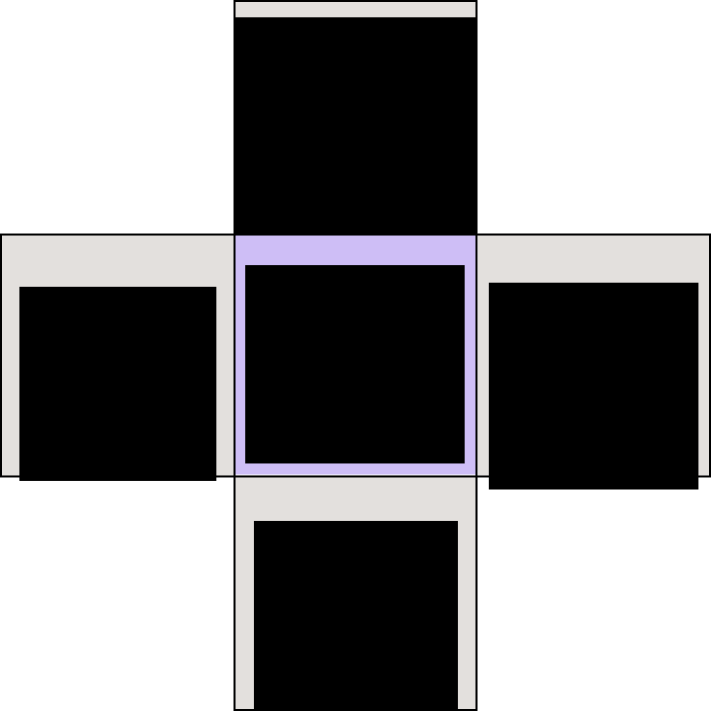
\includegraphics[width=0.4\textwidth]{./pics/problem.pdf}
% problem.pdf: 0x0 pixel, 300dpi, 0.00x0.00 cm, bb=


There are three main Problems based on that:

 \begin{itemize}
  \item Agents often maintain their own state and data
  \item Interactive agents provide their own user interface
  \item Systems evolve over time
 \end{itemize}
\end{multicols}

\note{Ann-Kathrin}


\end{frame}


\section{Solution}

\section{Structure}

\section{Dynamics}

\section{Known Uses}


%Dokument
%Wo soll das hin?!
\section{Resonbility}

\begin{frame}
 \frametitle{Resonbility}
 
 \begin{itemize}
  \item coordinate lower-level PAC agents
  \item Composes lower-level PAC agents to a single unit of higher abstractation
 \end{itemize}

 %\note{Anna}
\end{frame}


\end{document}
